\section{Funktionaler Vergleich der Spracherweiterungen}
\label{vergleich}

\subsection{Anforderungen an Spracherweiterungen}
\label{vergleich:anforderungen}

Ein Vergleich der Fähigkeiten der einzelnen Spracherweiterungen erfordert einen
Kriterienkatalog, anhand dessen die Bewertung erfolgen kann. Dabei sind sowohl
die Sicht auf die Daten, also der Umgang der Spracherweiterungen mit den Daten,
als auch die Sicht auf die Aufgaben, also die Transformation der Daten, zu
berücksichtigen.

\subsubsection{Datensicht}
\label{vergleich:anforderungen:datensicht}

Der effiziente Umgang mit großen Datenmengen ist seit jeher eines der
Kernprobleme des \gls{hpc} im Allgemeinen und heterogener Systeme im Besonderen,
d.h.\ unterschiedlicher Berechnungs-Hardware im selben Rechnersystem. Michael
Wong\footnote{Mitglied des C++-Standard-Komitees, ehemaliger Projektleiter des
XL-C++-Compilers der Firma IBM und derzeit Entwicklungsleiter des Unternehmens
Codeplay, das unter anderem den SYCL-Standard implementiert} bezeichnete in
einem Vortrag im November 2018 vor LLVM-Entwicklern die folgenden Punkte als
essentielle Probleme der Programmierung heterogener Systeme
(vgl.~\cite{wong2018}):

\paragraph{Datenbewegung} 
Die Bewegung der Daten ist stets mit Kosten verbunden. Im Allgemeinen ist damit
der Zeitbedarf gemeint, um Daten etwa vom Hauptspeicher des Systems in den
Speicher der GPU zu kopieren. Im weiteren Sinne kann dieser Punkt aber auch
andere Kriterien umfassen, wie z.B.\ den für den Kopiervorgang notwendigen
Energiebedarf, der als Bestandteil des gesamten Energiebedarfs von
\gls{hpc}-Systemen in jüngerer Zeit ebenfalls Gegenstand der Forschung geworden
ist.

Aus der Sicht des Programmierers ist außerdem die Frage relevant, ob die
Datenbewegung \textit{explizit} oder \textit{implizit} erfolgt. Die
\textit{explizite} Datenbewegung hat den Vorteil, dass der Programmierer
jederzeit die volle Kontrolle über die Verschiebung und damit auch über die
Performanz hat, geht jedoch mit einer höheren Programmierkomplexität und damit
Fehleranfälligkeit einher. Überdies wird die volle Kontrolle nicht
notwendigerweise an jeder Stelle gebraucht und bläht damit den Quelltext unnötig
auf. Die Adressräume bleiben bei der expliziten Datenbewegung getrennt (siehe
Abbildung~\ref{vergleich:anforderungen:datensicht:explizitebewegung})

Diesem Ansatz steht die \textit{implizite} Datenbewegung gegenüber. Diese
überlässt den Zeitpunkt und den konkreten Vorgang des Kopierens oder
Verschiebens sowie den Umfang der bewegten Datenmenge der Laufzeitumgebung; aus
Sicht des Programmierers existiert ein virtueller Adressraum, den sich CPU und
GPU teilen (siehe
Abbildung~\ref{vergleich:anforderungen:datensicht:implizitebewegung}).

\begin{figure}[!hbt]
    \centering
    \begin{subfigure}{0.75\textwidth}
        \centering
        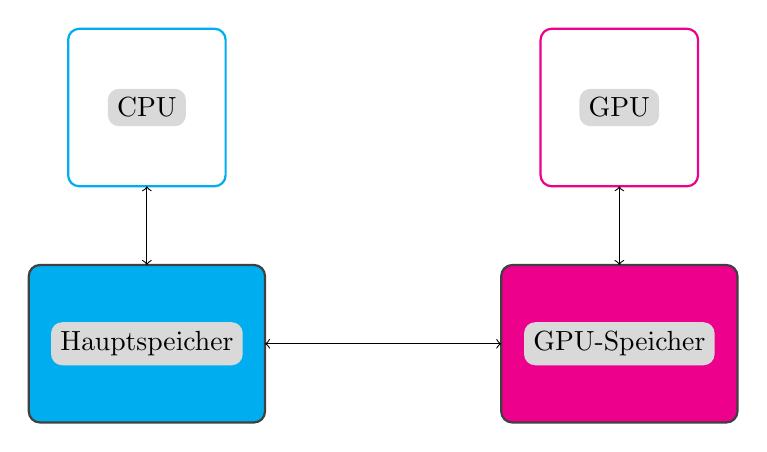
\begin{tikzpicture}
            \draw [thick, rounded corners, draw = cyan]
                  (-1.0, 0.0) rectangle (1.0, 2.0) node[pos = 0.5]
                  {CPU};

            \draw [thick, rounded corners, fill = cyan, draw = darkgray]
                  (-1.5, -3.0) rectangle (1.5, -1.0) node[pos = 0.5]
                  {Hauptspeicher};

            \draw [thick, rounded corners, draw = magenta]
                  (5.0, 0.0) rectangle (7.0, 2.0) node[pos=0.5] {GPU};

            \draw [thick, rounded corners, fill = magenta, draw = darkgray]
                  (4.5, -3.0) rectangle (7.5, -1.0) node[pos = 0.5]
                  {GPU-Speicher};

            \draw [<->] (0.0, 0.0) -- (0.0, -1.0); % CPU <-> RAM
            \draw [<->] (6.0, 0.0) -- (6.0, -1.0); % GPU <-> GPU-RAM
            \draw [<->] (1.5, -2.0) -- (4.5, -2.0); % RAM <-> GPU-RAM
        \end{tikzpicture}
        \caption{Sicht auf den Adressraum bei expliziter Datenbewegung.}
        \label{vergleich:anforderungen:datensicht:explizitebewegung}
    \end{subfigure}
    \par\bigskip
    \begin{subfigure}{0.75\textwidth}
        \centering
        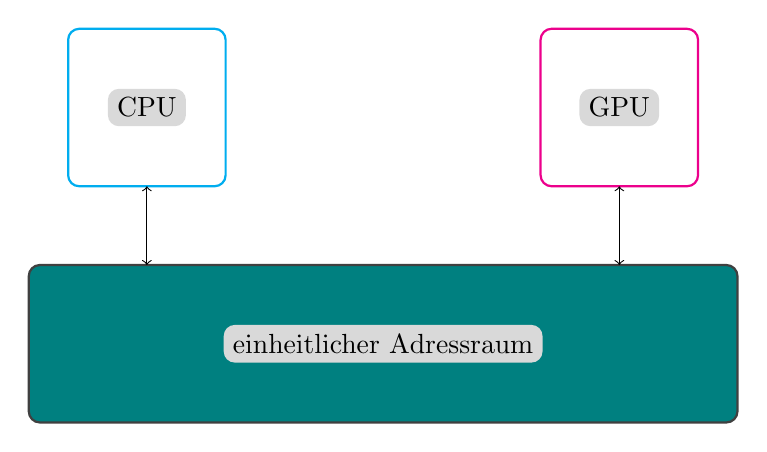
\begin{tikzpicture}
            \draw [thick, rounded corners, draw = cyan]
                  (-1.0, 0.0) rectangle (1.0, 2.0) node[pos = 0.5]
                  {CPU};

            \draw [thick, rounded corners, draw = magenta]
                  (5.0, 0.0) rectangle (7.0, 2.0) node[pos=0.5] {GPU};

            \draw [thick, rounded corners, fill = teal, draw = darkgray]
                  (-1.5, -3.0) rectangle (7.5, -1.0) node[pos = 0.5]
                  {einheitlicher Adressraum};

            \draw [<->] (0.0, 0.0) -- (0.0, -1.0); % CPU <-> Adressraum
            \draw [<->] (6.0, 0.0) -- (6.0, -1.0); % GPU <-> Adressraum
        \end{tikzpicture}
        \caption{Sicht auf den Adressraum bei impliziter Datenbewegung.}
        \label{vergleich:anforderungen:datensicht:implizitebewegung}
    \end{subfigure}
    \caption{Verschiedene Adressraumsichten}
    \label{vergleich:anforderungen:datensicht:adressraeume}
\end{figure}

Eine bewertende Gegenüberstellung beider Ansätze übersteigt den Rahmen dieser
Arbeit (und ist bisher auch in der Literatur nicht zu finden). Stattdessen wird
untersucht, in welcher Form beide Ansätze von den jeweiligen Spracherweiterungen
unterstützt werden.

\paragraph{Datenanordnung}

Die Anordnung der Daten im Speicher kann aufgrund einer Reihe von Faktoren, wie
etwa unterschiedlicher optimaler Zugriffsmuster von CPUs (\textit{cachelines})
und GPUs (\textit{strided access}), erheblich zur Performanz der Berechnung
beitragen. Aus Sicht des Programmieres ist es daher wünschenswert, dass die
Spracherweiterung eine abstrakte Sicht auf den von ihr verwendeten Speicher
bietet, welche die optimalen Zugriffsmuster der verschiedenen Hardware kapselt.

\paragraph{Datenaffinität}

Die Datenaffinität definiert die Zuordnung und Nähe eines Speicherbereichs zu
einer \textit{bestimmten} Ausführungseinheit, die auf diesen Speicherbereich
zugreifen muss. Im Hinblick auf GPUs meint dies die Zuordnung von im
Hauptspeicher liegenden Daten auf eine oder mehrere GPUs.

\paragraph{Datenlokalität}

Die obigen Punkte sind alle eng mit dem Aspekt der Datenlokalität verknüpft.
Im GPU-Kontext ist vornehmlich relevant, inwiefern sich die einzelnen
Ebenen der Speicherhierarchie (globaler Speicher der GPU, lokaler Speicher und
Cache der auf der GPU verbauten parallelen Prozessoren, Register der einzelnen
Threads) durch die Spracherweiterungen ansteuern und nutzen lassen.

\subsubsection{Aufgabensicht}
\label{vergleich:anforderungen:aufgabensicht}

Die im vorherigen Abschnitt genannten Punkte stellen die in dieser Arbeit
verwendeten Vergleichskriterien dar, bedürfen jedoch noch einer Ergänzung:

\paragraph{Aufgabengraphen}

Die Abfolge und Abhängigkeiten einzelner \textit{Kernel} lassen sich in Form
eines Graphen darstellen (siehe
Abbildung~\ref{vergleich:anforderungen:aufgabensicht:graph}). Eine effiziente
Ausnutzung der Parallelität voneinander unabhängiger Aufgaben setzt voraus,
dass Kernel \textit{asynchron} -- sowohl im Hinblick auf die CPU als auch
untereinander -- und \textit{parallel} auf der gleichen GPU ausgeführt werden
können. Im Rahmen dieser Arbeit wird deshalb ebenfalls untersucht, welche Mittel
die einzelnen Spracherweiterungen zur Verfügung stellen, um Aufgabengraphen zu
implementieren.

\begin{figure}[htb]
    \centering
    \begin{tikzpicture}
        \tikzstyle{every node} = [node distance = 3cm, fill = gray!30]

        \Vertex{B}
        \NOEA(B){A}
        \SOEA(B){D}
        \NOEA(D){C}

        \tikzstyle{EdgeStyle}=[post]
        \Edge(A)(B)
        \Edge(A)(C)
        \Edge(B)(D)
        \Edge(C)(D)
    \end{tikzpicture}
    \caption{Beispielhafter Aufgabengraph. Der Kernel D hängt von den Kerneln
             B und C ab, die voneinander unabhängig sind, jedoch beide vom
             Kernel A abhängen.}
    \label{vergleich:anforderungen:aufgabensicht:graph}
\end{figure}

\subsection{CUDA}
\label{vergleich:cuda}

\subsubsection{Einführung}
\label{vergleich:cuda:einfuehrung}

Da der CUDA-Compiler \texttt{nvcc} ein C++-Compiler ist, lässt sich CUDA neben
C++ auch in klassischen C-Programmen nutzen, sofern die Inkompatibilitäten
zwischen C und C++ beachtet werden. Zu diesem Zweck ist das \gls{api} auf
C-Konventionen beschränkt und unterstützt C++-Idiome nur sehr begrenzt. Die
CUDA-Kernel selbst werden in einem C++-Dialekt geschrieben.
(vgl.~\cite{cudaguide}, Abschnitt F)

CUDA-Kernel werden gemeinsam mit dem sie aufrufenden Quelltext kompiliert; CUDA
folgt damit dem Modell der \textit{\gls{singlesource}}\footnote{CUDAs frühester
Konkurrent \gls{opencl} kompiliert die Device-Kernel dagegen erst zur Laufzeit
des Programms, um zwischen verschiedenen Architekturen portabel zu bleiben
(\textit{\gls{splitsource}}.)}. \texttt{nvcc} extrahiert dazu die Kernel und
Device-Funktionen aus dem Quelltext und reicht den verbleibenden C- oder
C++-Quelltext an den auf dem System befindlichen entsprechenden Compiler
weiter. Der Device-Quelltext wird in einem weiteren Schritt vom tatsächlichen
Device-Compiler \texttt{cicc} in die Maschinensprache der Ziel-GPU übersetzt.

Der Quelltext~\ref{vergleich:cuda:einfuehrung:vecadd} zeigt einen
Beispiel-Kernel in CUDA. Das Schlüsselwort \texttt{\_\_global\_\_} markiert
einen Kernel, der vom Compiler extrahiert und für das Device übersetzt wird. Mit
dem Schlüsselwort \texttt{\_\_device\_\_} werden Funktionen markiert, die
innerhalb eines Kernels aufgerufen werden können, selbst jedoch keine
eigenständigen Kernel darstellen. Die letzte Zeile zeigt den Aufruf des Kernels
aus dem Host-Code heraus. Die hier sichtbaren Konzepte der Blocks und Threads
werden in den nächsten Abschnitten ausführlich erklärt.

\begin{code}
    \begin{minted}[breaklines,breakafter=\,,escapeinside=||,fontsize=\small]{cuda}
__device__ int foo() { /* ... */ }
__global__ void vec_add(const float* a, const float* b, float* c,
                        std::size_t dim)
{
    auto i = blockIdx.x * blockDim.x + threadIdx.x;
    if(i < dim) return;

    auto k = foo();
    c[i] = a[i] + b[i] + k;
}

vec_add<<<block_num, thread_num>>>(dev_a, dev_b, dev_c, dim);
    \end{minted}
    \caption{Beispielkernel in CUDA}
    \label{vergleich:cuda:einfuehrung:vecadd}
\end{code}


\subsubsection{Ausführungsmodell}

Ein \textit{thread} ist die kleinste selbstständige Einheit, die eine Aufgabe
ausführen kann und direkt auf einen Hardware-Thread eines Multiprozessors
abbildbar. \textit{Threads} sind auf der Hardware-Ebene in \textit{warps}
 -- bestehend aus 32 \textit{threads} -- zusammengefasst, die
 synchron\footnote{Die neuen
Architekturen seit Volta können mit weniger als 32 \textit{threads} besser
umgehen als die Vorgängerarchitekturen. Möglich wird dies durch ein Verfahren
namens \textit{independent thread scheduling}, das diese Hardware-Limitierung
teilweise aufhebt.} auch unterhalb dieser Grenze dieselben Instruktionen
ausführen. \textit{Warps} entsprechen damit Registern der CPU, die das Modell
\gls{simd} unterstützen, sind im Vergleich zu diesen allerdings flexibler
programmierbar. Dieses Hardware-Modell wird von NVIDIA auch als \gls{simt}
bezeichnet.

Die nächsthöhere Ebene bilden \textit{blocks}, die aus bis zu \num{1024}
\textit{threads} in drei Dimensionen bestehen können (das Produkt der
\textit{thread}-Zahl in $x$-, $y$- und $z$-Richtung darf \num{1024} also nicht
übersteigen). Während die Anzahl der \textit{threads} in diesem Rahmen frei
wählbar ist, bedingt die feste \textit{warp}-Größe, dass eine
\textit{block}-Größe ein Vielfaches von 32 sein sollte. Andernfalls könnte
der letzte \textit{warp} jedes \textit{blocks} nicht vollständig genutzt werden,
was zu geringerer Parallelität auf \textit{thread}-Ebene führen würde. Ein
\textit{block} wird genau einem Multiprozessor zugeordnet und von diesem
ausgeführt. Sind mehr \textit{blocks} als Multiprozessoren vorhanden, werden
\textit{blocks}, die z.B.\ durch Speicherzugriffe blockiert sind, vom Scheduler
in einen wartenden Zustand versetzt und durch wartende, aber bereite
\textit{blocks} ersetzt. Dieser Kontextwechsel geschieht auf einer GPU bei einer
geringen Anzahl von \textit{blocks} pro Multiprozessor deutlich schneller als
auf einer CPU und ist mit nur wenigen Zyklen verbunden, da die verwendeten
Register und Caches nicht geleert und im Speicher hinterlegt werden müssen. Eine
zu hohe Zahl von \textit{blocks} pro Multiprozessor kann im Umkehrschluss einen
gegenteiligen Effekt hervorrufen, durch den der Kontextwechsel nicht mehr derart
performant ist.

Alle \textit{threads} eines \textit{blocks} können untereinander über den
Speicher des Multiprozessors kommunizieren (\textit{shared memory}). Barrieren
ermöglichen die Synchronisation zwischen \textit{warps}, während
\textit{threads} innerhalb eines \textit{warps} durch spezielle Intrinsiken
kommunizieren können.

Die Gesamtheit der \textit{blocks} bildet das \textit{grid}, das ebenfalls bis
zu drei Dimensionen umfassen kann. Eine Synchronisierung zwischen
\textit{blocks} ist mit CUDA selbst nicht möglich, allerdings ermöglicht
das im Zusammenhang mit CUDA 9 eingeführte (vgl.~\cite{cuda2018}, S.\ 3)
\gls{api} \textit{cooperative groups} eine \textit{grid}-weite Barriere.
(vgl.~\cite{cudaguide}, Abschnitt 2.2)

\subsubsection{Datensicht}
\label{vergleich:cuda:datensicht}

\paragraph{Datenbewegung}

CUDA bietet mehrere Möglichkeiten der Datenbewegung an. Die \textit{explizite}
Datenbewegung wird seit der ersten CUDA-Version unterstützt und erfordert vom
Programmierer die Allokation von Host- und Device-Speicher, das Auslösen des
Kopiervorgangs der Daten vom Host auf das Device (und zurück) und das Freigeben
des Speichers, wenn er nicht mehr benötigt wird (siehe
Quelltext~\ref{vergleich:cuda:datensicht:explizitebewegung}).

\begin{code}
    \begin{minted}[breaklines,breakafter=\,,escapeinside=||,fontsize=\small]{c++}
auto a_h = new float[num_elems];
auto b_h = new float[num_elems];

/* a_h initialisieren */

auto a_d = static_cast<float*>(nullptr);
auto b_d = static_cast<float*>(nullptr);
cudaMalloc(&a_d, num_elems * sizeof(float));
cudaMalloc(&b_d, num_elems * sizeof(float));

cudaMemcpy(a_d, a_h, num_elems * sizeof(float),
           |\textbf{\textcolor{keyword-green}{cudaMemcpyHostToDevice}}|);

kernel<<<...>>>(a_d, b_d, num_elems);

cudaMemcpy(b_h, b_d, num_elems * sizeof(float),
           |\textbf{\textcolor{keyword-green}{cudaMemcpyDeviceToHost}}|);

cudaFree(b_d);
cudaFree(a_d);

delete[] b_h;
delete[] a_h;
    \end{minted}
    \caption{Explizite Datenbewegung mit CUDA}
    \label{vergleich:cuda:datensicht:explizitebewegung}
\end{code}

Seit dem im Jahr 2011 erschienenen CUDA 4 unterstützt CUDA einen einheitlichen
virtuellen Adressraum für Host und Device (vgl.~\cite{cuda2011}, S.\ 4). Dieser
ermöglichte noch keine implizite Datenbewegung, ersparte dem Programmierer
aber die Angabe der Kopierrichtung beim Aufruf von
\mintinline{c++}{cudaMemcpy}. Der letzte Parameter des Befehls konnte seit
diesem Zeitpunkt durch \mintinline{c++}{cudaMemcpyDefault} ersetzt werden.

Die \textit{implizite} Datenbewegung wird seit dem im Jahr 2014 erschienenen
CUDA 6 unterstützt (vgl.~\cite{cuda2014}, S.\ 3). Der Befehl
\mintinline{c++}{cudaMallocManaged} allokiert einen Speicherbereich, der sowohl
vom Host als auch vom Device angesteuert werden kann. Die CUDA-Laufzeitumgebung
sorgt dann im Hintergrund für das Kopieren der notwendigen Speicherbereiche. Es
obliegt jedoch dem Programmierer, die Synchronisierung zwischen Host und Device
auszuführen. Das in Quelltext~\ref{vergleich:cuda:datensicht:explizitebewegung}
aufgeführte Beispiel wird dadurch zu der in
Quelltext~\ref{vergleich:cuda:datensicht:implizitebewegung} gezeigten
Vereinfachung.

\begin{code}
    \begin{minted}[breaklines,breakafter=\,,escapeinside=||,fontsize=\small]{c++}
auto a = static_cast<float*>(nullptr);
auto b = static_cast<float*>(nullptr);

cudaMallocManaged(&a, num_elems * sizeof(float));
cudaMallocManaged(&b, num_elems * sizeof(float));

kernel<<<...>>>(a, b, num_elems);

cudaDeviceSynchronize();

/* b ab hier auf dem Host nutzbar */

cudaFree(b);
cudaFree(a);
    \end{minted}
    \caption{Implizite Datenbewegung ab CUDA 6}
    \label{vergleich:cuda:datensicht:implizitebewegung}
\end{code}

Im Jahr 2016 führte NVIDIA die Pascal-Architektur und CUDA 8 ein. Mit dieser
neuen Architektur wurde die implizite Datenbewegung weiter vereinfacht, da es
nun möglich war, gänzlich auf CUDA zur Speicherallokation zu verzichten: der
Aufruf von \mintinline{c++}{new} oder \mintinline{c}{malloc} genügt
(vgl.~\cite{harris2016}). Dadurch wurde auch die Verwendung von C++-Containern
im Zusammenhang mit CUDA einfacher, deren Speicherbereich man nun direkt an
CUDA-Kernel übergeben konnte (siehe
Quelltext~\ref{vergleich:cuda:datensicht:explizitcuda8}).

\begin{code}
    \begin{minted}[breaklines,breakafter=\,,escapeinside=||,fontsize=\small]{c++}
auto a = std::vector<float>{};
auto b = std::vector<float>{};

a.resize(num_elems);
b.resize(num_elems);

kernel<<<...>>>(a.data(), b.data(), num_elems);

cudaDeviceSynchronize();

/* b ab hier auf dem Host nutzbar */
    \end{minted}
    \caption{Implizite Datenbewegung ab CUDA 8 und Pascal}
    \label{vergleich:cuda:datensicht:explizitcuda8}
\end{code}

\paragraph{Datenanordnung}

Die Anordnung der Daten im globalen Speicher der GPU entspricht bei der
Allokation mit \mintinline{c++}{cudaMalloc} und der Kopie mit
\mintinline{c++}{cudaMemcpy} der Anordnung der Daten im Host-Speicher. Es ist
Aufgabe des Programmierers, die Effizienz der Anordnung und des
Zugriffsverhaltens sicherzustellen (vgl.~\cite{cudaguide}, Abschnitt 5.3.2,
Überschrift \glqq Global Memory\grqq).

Einen Sonderfall stellen zweidimensionale Arrays dar. Die Adresse $A$ eines
Felds eines 2D-Arrays mit der Startadresse $S$ und der Breite $B$ durch einen
Thread mit den Koordinaten $(x, y)$ berechnet sich in vielen Anwendungsfällen
wie folgt:

\begin{align*}
    A = S + y * B + x
\end{align*}

Ein effizienter Zugriff dieser Form erfordert sowohl eine Block-Breite als auch
eine Array-Breite, die ein mathematisches Vielfaches der Warpbreite sind. Mit
\mintinline{c++}{cudaMallocPitch} und \mintinline{c++}{cudaMemcpy2D} kann man
letzterer Anforderung Rechnung tragen. Eine Erweiterung dieses Prinzips auf
dreidimensionale Arrays, die man sich auch als Array von 2D-Arrays vorstellen
kann, ist mit \mintinline{c++}{cudaMalloc3D} und \mintinline{c++}{cudaMemcpy3D}
möglich. (vgl.~\cite{cudaguide}, Abschnitt 5.3.2, Überschrift \glqq
Two-Dimensional Arrays\grqq)

Sofern häufig auf benachbarte Spalten und Zeilen eines Arrays zugegriffen
wird, lässt sich dies effizienter auslesen, wenn die eigentlich für
Grafikoperationen -- die häufig benachbarte Pixel manipulieren -- vorgesehenen
Textur-Caches der GPU genutzt werden. Eine für diese Caches optimale
Speicheranordnung lässt sich mit \mintinline{c++}{cudaMallocArray}
bewerkstelligen. Ein auf diese Weise angelegtes \mintinline{c++}{cudaArray} ist
kein Zeiger, sondern eine für den Programmierer opake Datenstruktur, auf die
nur über spezielle Texturbefehle zugegriffen werden kann.
(vgl.~\cite{cudaguide}, Abschnitt 5.3.2, Überschrift \glqq Texture and Surface
Memory\grqq)

\paragraph{Datenaffinität}

Die explizite Datenbewegung ordnet die kopierten Daten automatisch der
\textit{aktiven} GPU zu. Der CUDA-Kontext kennt generell nur ein aktives Device;
will man in einem Multi-GPU-System auf eine andere GPU wechseln, geschieht dies
durch den manuellen Wechsel mit dem Befehl \texttt{cudaSetDevice} (siehe
Quelltext~\ref{vergleich:cuda:datensicht:setdevice}).

Dieses Verfahren gilt zum Teil auch für die implizite Datenbewegung. Speicher,
der mit dem Befehl \texttt{cudaMallocManaged} reserviert wurde, wird bei allen
NVIDIA-GPU-Architekturen bis einschließlich \textit{Maxwell} nur zwischen dem
Host und dem zum Zeitpunkt der Reservierung aktiven Device ausgetauscht. Ab der
\textit{Kepler}-Architektur wird der Speicher dagegen auf allen GPUs sichtbar
und nach Bedarf auf die GPU kopiert, welche die Daten benötigt.
(vgl.~\cite{cudaguide}, Abschnitt K.1.5)

\begin{code}
    \begin{minted}[fontsize=\small]{c++}
auto count = 0;
cudaGetDeviceCount(&count); // Zahl der GPUs abfragen

cudaSetDevice(0); // Device 0 aktiv
cudaMemcpy(..., cudaMemcpyHostToDevice); // kopieren auf Device 0

cudaSetDevice(1); // Device 1 aktiv
cudaMemcpy(..., cudaMemcpyHostToDevice); // kopieren auf Device 1
    \end{minted}
    \caption{Setzen der aktiven GPU mit CUDA}
    \label{vergleich:cuda:datensicht:setdevice}
\end{code}

\paragraph{Datenlokalität}

CUDA kennt sieben Ebenen innerhalb der GPU-Speicherhierarchie
(vgl.~\cite{cudaguide}, Abschnitt 5.3.2).

\textit{Global memory} ist der Hauptspeicher der GPU und für alle
Multiprozessoren sichtbar. Die Zugriffe sind jedoch zeitaufwendig.

Zugriffe auf den \textit{global memory} erfolgen über L1- (pro Multiprozessor)
und L2-Caches (alle Multiprozessoren). Die Caches lassen sich vom Programmierer
nicht direkt ansteuern.

\textit{Constant memory} liegt im \textit{global memory}, wird aber auf eine
spezielle Weise in den Cache geladen. Er ermöglicht deutlich schnellere
Speicherzugriffe, wenn alle \textit{threads} eines \textit{warps} gleichzeitig
auf dasselbe Datum zugreifen.

Operationen, die die Textureinheiten der GPU verwenden, können über die
Textur-Caches der GPU lesend auf den \textit{global memory} zugreifen. Diese
Caches sind für häufige zweidimensionale Speicherzugriffe auf benachbarte Zeilen
und Spalten optimiert. Sie sind vom Programmierer mittels der Intrinsik
\texttt{\_\_ldg} direkt ansprechbar oder können implizit durch die in CUDA
enthaltenen Texturbefehle genutzt werden.

\textit{Shared memory} ist ein spezieller L1-Cache, der direkt vom Programmierer
lesbar und beschreibbar ist. Der \textit{shared memory} ist in seiner Kapazität
sehr eingeschränkt (er umfasst nur einige KiB), ermöglicht dem Programmierer
aber sehr schnelle Zugriffe sowie die Kommunikation zwischen \textit{threads}
eines \textit{blocks}.

Die Register des Multiprozessors werden \textit{threads} nach Bedarf zugeordnet
und sind vom Programmierer nicht direkt ansprechbar.

\textit{Local memory} ist \textit{thread}-lokaler \textit{global memory}. In
diesem werden lokale Variablen, die nicht mehr in die Register passen
(weil deren Anzahl erschöpft ist), oder Arrays unbekannter Länge automatisch
untergebracht. Da der \textit{local memory} versteckt im \textit{global memory}
liegt, ist seine Nutzung aufgrund der langen Zugriffszeiten üblicherweise
unerwünscht.

\subsubsection{Aufgabensicht}

\paragraph{Aufgabengraphen}

Aufgabengraphen lassen sich in CUDA auf zwei Arten implementieren. Der
herkömmliche Weg ist die Verwendung von \textit{streams}. Diese können als
Warteschlangen für Aufgaben (Speicherbewegungen, Kernel-Ausführungen) gesehen
werden und sind untereinander und in Bezug auf den Host asynchron. Das heißt,
dass verschiedene Kernel in getrennten \textit{streams} parallel auf der GPU
ausgeführt werden können (entsprechende Hardware-Ressourcen vorausgesetzt).
Innerhalb eines \textit{streams} sind alle Aufgaben immer serialisiert, zwei
Kernel im selben \textit{stream} werden also immer nacheinander ausgeführt.

Die Kommunikation bzw.\ Synchronisation zwischen \textit{streams} erfolgt über
\textit{events}. \textit{Events} werden z.B.\ durch das Beenden eines Kernels
ausgelöst. Ist ein Kernel eines anderen \textit{streams} von diesem abhängig,
lässt sich durch das Warten auf dieses \textit{event} der \textit{stream}
blockieren, bis die Ausführung fortgesetzt werden kann.

Der Quelltext~\ref{vergleich:cuda:aufgabensicht:streams} zeigt die
Implementierung des Beispiel-Graphen
in Abbildung~\ref{vergleich:anforderungen:aufgabensicht:graph} mit
\textit{streams}.

\begin{code}
    \begin{minted}[fontsize=\small]{c++}
A<<<..., stream1>>>();
// eventA wird ausgelöst, sobald A fertig ist
cudaEventRecord(eventA, stream1);

B<<<..., stream1>>>(); // wartet automatisch auf A

// stream2 wartet auf eventA
cudaStreamWaitEvent(stream2, eventA);
// C kann jetzt ausgeführt werden
C<<<..., stream2>>>();
// eventC wird ausgelöst, sobald C fertig ist
cudaEventRecord(eventC, stream2);

// stream1 wartet auf eventC
cudaStreamEvent(stream1, eventC);
D<<<..., stream1>>>(); // wartet automatisch auf B
    \end{minted}
    \caption{Aufgabengraph mit \textit{streams}}
    \label{vergleich:cuda:aufgabensicht:streams}
\end{code}

Der \textit{stream}-Ansatz hat den Nachteil, dass bei iterativen Verfahren, die
das mehrfache Ausführen des Graphen erfordern, durch das ständige Starten der
Kernel und das manuelle Blockieren der \textit{streams} viel Overhead erzeugt
wird. Die mit dem 2018 veröffentlichten CUDA 10 eingeführten
\textit{CUDA Graphs} (vgl.~\cite{cuda10rel}, S.\ 4) sollen dieses Problem lösen
(vgl.~\cite{ramarao2018} für eine Einführung).

Aufgabengraphen lassen sich mit diesem \gls{api} direkt implementieren.
Quelltext~\ref{vergleich:cuda:aufgabensicht:graph} zeigt die
Abbildung~\ref{vergleich:anforderungen:aufgabensicht:graph} entsprechende
Implementierung. 

\begin{code}
    \begin{minted}[fontsize=\small]{c++}
cudaGraphCreate(&graph);

// Abhängigkeiten definieren
cudaGraphAddNode(graph, A, {}, ...);
cudaGraphAddNode(graph, B, {A}, ...);
cudaGraphAddNode(graph, C, {A}, ...);
cudaGraphAddNode(graph, D, {B, C}, ...);

// Graph-Instanz erzeugen
cudaGraphInstantiate(&instance, graph);

// Graph-Instanz auf stream ausführen
cudaGraphLaunch(instance, stream);
    \end{minted}
    \caption{Aufgabengraph mit \textit{CUDA Graphs}}
    \label{vergleich:cuda:aufgabensicht:graph}
\end{code}

\subsection{HIP}

\subsubsection{Einführung}

AMDs \gls{hip}-\gls{api} ist als portable Alternative zu CUDA gedacht und de
facto ein Klon des CUDA-\gls{api}, bei dem fast jeder CUDA-Befehl
\texttt{cudaCmd} seine genaue Entsprechung im \gls{hip}-Befehl \texttt{hipCmd}
findet. Tatsächlich werden \gls{hip}-Quelltexte, die für eine NVIDIA-GPU
kompiliert werden sollen, wieder in CUDA-Quelltexte umgewandelt, da die
\gls{hip}-Befehle die äquivalenten CUDA-Befehle ohne Umwege aufrufen.

Die in den vorherigen Abschnitten für CUDA dargestellten Prinzipien gelten daher
weitestgehend auch für \gls{hip}; vorhandene Unterschiede werden in den
folgenden Abschnitten aufgeführt.

\gls{hip} für AMD-GPUs ist eine dünne Schicht über AMDs eigentlichem
\gls{gpgpu}-\gls{api}, \gls{hc}, das in Abschnitt~\ref{vergleich:hc} vorgestellt
wird.

Der Quelltext~\ref{vergleich:hip:einfuehrung:vecadd} zeigt einen in HIP
geschriebenen Beispielkernel und den zugehörigen Aufruf innerhalb des
Host-Codes. Die Block- und Threadkonzepte entsprechen den in CUDA vorhandenen.

\begin{code}
    \begin{minted}[breaklines,breakafter=\,,escapeinside=||,fontsize=\small]{cuda}
__device__ int foo() { /* ... */ }

__global__ void vec_add(const float* a, const float* b, float* c,
                        std::size_t dim)
{
    auto i = |\textcolor{keyword-green}{hipBlockIdx\_x}| * |\textcolor{keyword-green}{hipBlockDim\_x}| + |\textcolor{keyword-green}{hipThreadIdx\_x}|;
    if(i < dim) return;

    auto k = foo();
    c[i] = a[i] + b[i] + k;
}

hipLaunchKernelGGL(vec_add, block_num, thread_num, 0, 0,
                   dev_a, dev_b, dev_c, dim);
    \end{minted}
    \caption{Beispielkernel in HIP}
    \label{vergleich:hip:einfuehrung:vecadd}
\end{code}

\subsubsection{Datensicht}

\paragraph{Datenbewegung}

Die implizite Datenbewegung, die mit \texttt{cudaMallocManaged} möglich ist,
hat gegenwärtig kein \gls{hip}-Äquivalent. Programmierer haben daher nur die
Möglichkeit der expliziten Datenbewegung.

\paragraph{Datenanordnung}

Zweidimensionaler Speicher kann auf CUDA-GPUs mit \texttt{cudaMallocPitch} in
einer optimierten Anordnung reserviert werden. Dieser Befehl wird derzeit nicht
in \gls{hip} abgebildet. Gleiches gilt für \texttt{cudaArray}s, die in ihrer
Anordnung für den Textur-Cache optimiert sind.

\paragraph{Datenlokalität}

Die Textur-Einheiten und damit der Textur-Cache der GPU werden von \gls{hip} zur
Zeit nur eingeschränkt unterstützt.

\subsubsection{Aufgabensicht}

\paragraph{Aufgabengraphen}

Aufgabengraphen lassen sich in \gls{hip} nur über \textit{streams}
implementieren, \textit{CUDA Graphs} werden momentan nicht unterstützt.

\subsection{HC}
\label{vergleich:hc}

\subsubsection{Einführung}

AMDs \gls{hc}-\gls{api} ist ein Dialekt des C++AMP-API, das im August 2012 von
der Firma Microsoft veröffentlicht wurde. C++AMP setzte auf der
Grafikschnittstelle DirectX 11 auf und ermöglichte die direkte Programmierung
von GPUs und CPU-\gls{simd}-Registern mittels C++. 2013 übernahm AMD C++AMP
für sein \gls{hsa}-Programm und erweiterte das API um AMD-spezifische Funktionen
und GPU-relevante Features.

HC-Kernel können entweder als separate Funktionen oder Funktoren geschrieben 
oder als Lambda-Funktionen direkt in den C++-Quelltext eingebettet werden. Der
Compiler extrahiert die Kernel aus dem sie umgebenden Quelltext und übersetzt
sie in den GPU-Maschinencode, während der restliche Quelltext in den
CPU-Maschinencode umgewandelt wird. Der komplette Quelltext wird also in einem
Schritt kompiliert.

Unglücklicherweise ist die Dokumentationslage des \gls{hc}-\gls{api} sehr
schlecht. Es gibt von AMD keine öffentlich zugänglichen Dokumente, die der
CUDA-Dokumentation in Umfang und Inhalt nahe kämen. Die in den folgenden
Abschnitten präsentierten Erkenntnisse basieren auf der unvollständigen
\gls{hc}-\gls{api}-Referenz, die ein AMD-Angestellter auf seiner privaten
GitHub-Seite zur Verfügung stellt (vgl.~\cite{hcref}), der C++AMP-Spezifikation
aus dem Jahr 2012\footnote{Die Features der Ende 2013 veröffentlichten
Spezifikation für C++AMP 1.2 werden von HC nicht unterstützt.}
(vgl.~\cite{cppamp2012}) und

Der Quelltext~\ref{vergleich:hc:einfuehrung:vecadd} zeigt einen in HC
geschriebenen Beispielkernel. Device-Funktionen und Kernel werden beide
mit dem Attribut \texttt{[[hc]]} markiert. Die letzten Zeilen zeigen den Aufruf
des Kernels innerhalb des Host-Codes. Auch hier werden die Konzepte in den
nächsten Abschnitten detailliert erklärt.

\begin{code}
    \begin{minted}[breaklines,breakafter=\,,escapeinside=||,fontsize=\small]{c++}
int foo() [[hc]] { /* ... */ }

void vec_add [[hc]] (hc::tiled_index<1> idx,
                     hc::array_view<const float> a,
                     hc::array_view<const float> b,
                     hc::array_view<float> c, std::size_t dim)
{
    auto i = idx.global[0];
    if(i < dim) return;

    auto k = foo();
    c[i] = a[i] + b[i] + k;
}

auto global_extent = hc::extent<1>{global_thread_num};
hc::parallel_for_each(global_extent.tile(tile_size),
[=](hc::tiled_index<1> idx)
{
    vec_add(idx, a_view, b_view, c_view, dim);
});
    \end{minted}
    \caption{Beispielkernel in HC}
    \label{vergleich:hc:einfuehrung:vecadd}
\end{code}

\subsubsection{Ausführungsmodell}

Das \gls{hc}-Ausführungsmodell ähnelt dem von CUDA sehr stark und unterscheidet
sich nur in einigen Details. Auch hier ist die kleinste Ausführungseinheit ein
\textit{thread}, die direkt auf einen Hardware-Thread eines Multiprozessors
abgebildet wird. Eine Gruppe von 64 \textit{Threads} bildet eine
\textit{wavefront} (das Gegenstück zu CUDA-\textit{warps}) und arbeitet synchron
die selben Instruktionen ab.

Auf der nächsthöheren Organisationsebene befinden sich \textit{tiles}, die
den CUDA-\textit{blocks} entsprechen und ebenfalls aus insgesamt \num{1024}
\textit{threads} bestehen können. Auch bei \gls{hc} ist die Größe der
\textit{tiles} bis zu dieser Grenze frei wählbar, wird aufgrund der
\textit{wavefront}-Größe in der Regel jedoch ein Vielfaches von 64 sein. Jede
\textit{tile} wird einem Multiprozessor zugeordnet und von diesem ausgeführt,
das Scheduling-Verhalten der GPU bei überzähligen \textit{tiles} entspricht
dem von CUDA.

Die \textit{threads} einer \textit{tile} teilen sich den Speicher eines
Multiprozessors, der \textit{tile static memory} genannt wird und CUDAs
\textit{shared memory} entspricht. Barrieren ermöglichen die Synchronisation
zwischen \textit{wavefronts}, zudem gibt es Hardware-Intrinsiken für die
Kommunikation innerhalb einer \textit{wavefront}.

CUDAs \textit{grid}-Konzept hat keine direkte \gls{hc}-Entsprechung, da
bei letzterem die Menge der \textit{tiles} keine große Rolle spielt. Stattdessen
ist die globale Problemgröße von Relevanz. Diese muss dabei nicht zwangsläufig
der Gesamtzahl der \textit{threads} entsprechen. Der Programmierer hat dadurch
die Möglichkeit, das Problem mit \textit{tiles} von selbst definierter Größe
zu bearbeiten oder nur die globale Problemgröße anzugeben und die Festlegung der
\textit{threads} und \textit{tiles} der Laufzeitumgebung zu überlassen.

\subsubsection{Datensicht}

\paragraph{Datenbewegung}

Die \textit{explizite} Datenbewegung geschieht über das Definieren des
Host-Speichers und eines GPU-Arrays sowie den anschließenden Aufruf des
\texttt{copy}-Befehls (siehe
Quelltext~\ref{vergleich:hc:datensicht:explizitebewegung}). Eine manuelle
Freigabe des Speichers ist nicht notwendig, da dies automatisch im Destruktor
des GPU-Arrays geschieht, sobald der umschließende Kontext verlassen wird.

\begin{code}
    \begin{minted}[breaklines,breakafter=\,,escapeinside=||,fontsize=\small]{c++}
auto a_h = std::vector<float>{};
auto b_h = std::vector<float>{};

a_h.resize(num_elems);
b_h.resize(num_elems);

/* a_h initialisieren */

auto a_d = hc::array<float, 1>{hc::extent<1>{num_elems}};
auto b_d = hc::array<float, 1>{hc::extent<1>{num_elems}};

hc::copy(std::begin(a_h), a_d);

hc::parallel_for_each( /* kernel */ );

hc::copy(b_d, std::begin(b_h))
    \end{minted}
    \caption{Explizite Datenbewegung mit HC}
    \label{vergleich:hc:datensicht:explizitebewegung}
\end{code}

Einen Mittelweg zwischen impliziter und expliziter Datenbewegung stellt die
direkte Zuordnung eines \texttt{hc::array} zu einem Datenbereich auf dem Host
dar. Die Host-Daten werden vollständig in das \texttt{hc::array} kopiert. Wenn
das System, auf dem das Programm ausgeführt wird, einen einheitlichen virtuellen
Speicherbereich unterstützt, ist das \texttt{hc::array} anschließend auch vom
Host aus ansprechbar (siehe Quelltext~\ref{vergleich:hc:datensicht:arraymix}).

\begin{code}
    \begin{minted}[breaklines,breakafter=\,,escapeinside=||,fontsize=\small]{c++}
auto a_h = std::vector<float>{};

a_h.resize(num_elems);

/* a_h initialisieren */

auto a_d = hc::array<float, 1>{hc::extent<1>{num_elems},
                               std::begin(a_h)};
auto b_d = hc::array<float, 1>{hc::extent<1>{num_elems},
                               std::begin(b_h)};

hc::parallel_for_each( /* kernel */ );

// wenn vom System unterstützt
func(b_d[42]);
    \end{minted}
    \caption{Implizite Datenbewegung mit HC-Arrays}
    \label{vergleich:hc:datensicht:arraymix}
\end{code}

Mit der \texttt{hc::array\_view}-Struktur ist eine weitere Möglichkeit der
\textit{impliziten} Datenbewegung gegeben. \texttt{hc::array\_view} lässt sich 
sowohl für ein \texttt{hc::array} als auch einen Standard-C++-Container
konstruieren. Die Bewegung der auf der jeweils anderen Seite benötigten Daten
geschieht im Verborgenen und nur für die tatsächlich angeforderten Teile, nicht
das gesamte Feld. Der Zugriff auf die Daten erfolgt dabei über die Methoden der
\texttt{hc::array\_view}, die einen internen Zwischenspeicher besitzt. Ein
Zugriff auf das original \texttt{hc::array} bzw.\ den originalen C++-Container
bedarf der vorherigen Synchronisierung (siehe
Quelltext~\ref{vergleich:hc:datensicht:implizitebewegung}). Darüber hinaus ist
zu bemerken, dass das ausführende System keinen einheitlichen virtuellen
Speicherbereich unterstützen muss, um \texttt{hc::array\_view} nutzen zu können.

\begin{code}
    \begin{minted}[breaklines,breakafter=\,,escapeinside=||,fontsize=\small]{c++}
auto a_h = std::vector<float>{};
a_h.resize(num_elems);

auto b_d = hc::array<float, 1>{hc::extent<1>{num_elems}};

/* a_h initialisieren */

auto a_view = hc::array_view<float, 1>{hc::extent<1>{num_elems}, a_h};
auto b_view = hc::array_view<float, 1>{b_d};

a_h[42] = ...;    // a_h schreiben
a_view.refresh(); // a_view synchronisieren

hc::parallel_for_each( /* kernel */ );

// a_view und b_view auf Host-Seite schreiben / lesen
for(auto i = 0; i < num_elems; ++i)
    a_view[hc::index<1>{i}] = b_view[hc::index<1>{i}];

a_view.synchronize(); // a_h synchronisieren
... = a_h[42]; // a_h enthält jetzt die neuen Daten
    \end{minted}
    \caption{Implizite Datenbewegung mit HC-Sichten}
    \label{vergleich:hc:datensicht:implizitebewegung}
\end{code}

\paragraph{Datenanordnung}

\texttt{hc::array} und \texttt{hc::array\_view} können bis zu drei Dimensionen
abdecken. Die interne Anordnung der Daten wird dabei vor dem Programmierer
verborgen. Dies wird einerseits daran deutlich, dass der Zugriff auf ein Feld
über den \texttt{[]}-Operator nicht durch ganze Zahlen erfolgt, sondern mittels
der speziellen Struktur \texttt{hc::index}, die ebenfalls bis zu drei
Dimensionen umfassen kann. Andererseits gibt es zwei Methoden, die den
gekapselten Zeiger zurückliefern:

\begin{itemize}
    \item \texttt{hc::array::accelerator\_pointer()} und das
          \texttt{hc::array\_view}-Gegenstück geben einen Zeiger auf den
          zugehörigen Device-Speicher zurück.
    \item \texttt{hc::array::data()} bzw. das
          \texttt{hc::array\_view}-Äquivalent liefern einen Zeiger auf ein
          \textit{linearisiertes} Array.
\end{itemize}

Aus den obigen Beobachtungen lässt sich daher folgern, dass die Anordnung der
Daten im GPU-Speicher nicht unbedingt der Anordnung im Hauptspeicher entsprechen
muss und sich unter Umständen auch zwischen verschiedenen \gls{hc}-Versionen
oder GPUs unterscheiden kann.

\paragraph{Datenaffinität}

Ein \texttt{hc::array} ist immer an ein bestimmtes Device gebunden. Sofern der
Programmierer bei der Konstruktion eines \texttt{hc::array}s in einem
Multi-GPU-System kein Device angibt, entscheidet die Laufzeitumgebung, auf
welcher GPU der Speicher reserviert wird. Über den \texttt{hc::copy}-Befehl
lassen sich Daten direkt zwischen \texttt{hc::array}s auf verschiedenen GPUs
bewegen (siehe Quelltext~\ref{vergleich:hc:datensicht:arrayaff}).

\begin{code}
    \begin{minted}[breaklines,breakafter=\,,escapeinside=||,fontsize=\small]{c++}
auto accelerators = hc::accelerator::get_all();

// Devices aussuchen
auto acc0 = ...;
auto acc1 = ...;

auto acc0_view = acc0.get_default_view();
auto acc1_view = acc1.get_default_view();
        
auto a_h = std::vector<float>{};
auto b_h = std::vector<float>{};
a_h.resize(num_elems);
b_h.resize(num_elems);

/* a_h und b_h initialisieren */

// a_d auf Device #0 anlegen
auto a_d = hc::array<float, 1>{hc::extent<1>{num_elems},
                               std::begin(a_h), acc0_view};

// b_d auf Device #1 anlegen
auto b_d = hc::array<float, 1>{hc::extent<1>{num_elems},
                               std::begin(b_h), acc1_view};

// Inhalt von a_d zu b_d kopieren
hc::copy(a_d, b_d);
    \end{minted}
    \caption{GPU-Speicheraffinität mit HC-Arrays}
    \label{vergleich:hc:datensicht:arrayaff}
\end{code}


\texttt{hc::array\_view} wird dagegen keiner GPU direkt zugeordnet. Bei einem
Zugriff auf den auf einer GPU liegenden und von \texttt{hc::array\_view}
verwalteten Speicher durch eine andere GPU wird der Prozess der Datenbewegung
grundsätzlich verborgen. Zu einem von ihm gewählten Zeitpunkt kann der
Programmierer den Vorgang jedoch durch den Befehl
\texttt{hc::array\_view::synchronize\_to()} auslösen.

\paragraph{Datenlokalität}

\gls{hc} unterscheidet lediglich zwei Ebenen innerhalb der Speicherhierarchie:

Der \textit{global memory} ist der auf dem Device vorhandene, allen
Multiprozessoren zugängliche Speicher. Er verfügt über ein großes
Fassungsvermögen, benötigt jedoch viel Zeit für Speicherzugriffe.

Die Multiprozessoren verfügen über programmierbare Caches, die von ihren
Hardware-Threads genutzt werden können. Dieser \textit{tile static memory}
genannte Speicher ist deutlich kleiner als der globale GPU-Speicher, kann jedoch
viel schneller angesteuert werden.

Obwohl \gls{hc} auf C++AMP basiert und hauptsächlich für GPUs und \gls{apu}s
gedacht ist, werden die in C++AMP enthaltenen (optionalen) Textur-Features nicht
unterstützt.

\subsubsection{Aufgabensicht}

\paragraph{Aufgabengraphen}

\gls{hc}-Kernel werden an Datenstrukturen vom Typ \texttt{hc::accelerator\_view}
übermittelt. Wie der Name impliziert, handelt es sich bei diesen Strukturen um
\textit{logische} Sichten auf einen Beschleuniger. Der Programmierer kann
mehrere \texttt{hc::accelerator\_view}s pro GPU erzeugen.

Alle Kernel, die einer bestimmten \texttt{hc::accelerator\_view} zugeordnet
werden, werden in der Reihenfolge ihrer Übermittlung ausgeführt. Kernel, die
zu verschiedenen Sichten gehören, können dagegen in anderer Reihenfolge oder
parallel ausgeführt werden. Die Synchronisation zwischen von einander abhängigen
Kerneln, die verschiedenen \texttt{hc::accelerator\_view}s übermittelt wurden,
erfolgt durch \texttt{hc::completion\_future}-Objekte. Diese entsprechen in
ihrem Verhalten weitestgehend den \texttt{std::future}-Objekten der
C++-Standardbibliothek, wurden jedoch um die Methode \texttt{then} erweitert,
die eine Ausführung eines nachfolgenden Befehls ermöglicht, sobald der aktuelle
Kernel beendet ist. Dieser Ansatz hat jedoch einen Nachteil: \texttt{then}
kann nur ein einziges Mal pro \texttt{completion\_future} ausgeführt werden,
eine Verkettung oder Parallelisierung mehrerer nachfolgender Befehle gestaltet
sich also recht schwierig.

Der Quelltext~\ref{vergleich:hc:aufgabensicht:views} zeigt die
Implementierung des Beispiel-Graphen
in Abbildung~\ref{vergleich:anforderungen:aufgabensicht:graph} mit
\gls{hc}.

Eine auf Graphen spezialisierte Schnittstelle existiert nicht.

\begin{code}
    \begin{minted}[breaklines,breakafter=\,,escapeinside=||,fontsize=\small]{c++}
auto accelerators = hc::accelerator::get_all();

auto acc = ...;
auto view0 = acc.create_view();
auto view1 = acc.create_view();
        
// A ausführen
auto futureA = hc::parallel_for_each(view0, /* kernel A */);

// B wird nach A ausgeführt
auto futureB = hc::parallel_for_each(view0, /* kernel B */);

// C ausführen, sobald A fertig ist
auto futureC = hc::completion_future{};
futureA.then([&]()
{
    futureC = hc::parallel_for_each(view1, /* kernel C */);
});

// D wird nach B ausgeführt, sobald C fertig ist
futureC.then([&]()
{
    hc::parallel_for_each(view0, /* kernel D */);
});
    \end{minted}
    \caption{Aufgabengraph mit HC}
    \label{vergleich:hc:aufgabensicht:views}
\end{code}


\subsection{SYCL}
\label{vergleich:sycl}

\subsubsection{Einführung}

Khronos' SYCL-Standard ging aus einer Compiler-Erweiterung der Firma Codeplay
hervor, die für den Einsatz auf PlayStation-3-Spielekonsolen konzipiert wurde.
Diese Erweiterung ermöglichte die Markierung von C++-Funktionen mit
Compiler-Direktiven, die dadurch automatisch auf den in der PlayStation 3
enthaltenen Beschleunigern ausgeführt wurden. (vgl.~\cite{lomueller2016})

SYCL ist syntaktisch vollständig mit dem C++-Standard kompatibel. Die Kernel
bedürfen also keiner speziellen Annotation, wie das etwa in CUDA mit der
Markierung \texttt{\_\_global\_\_} bzw.\ bei HC mit der Markierung
\texttt{[[hc]]} der Fall ist. Kernel werden als Lambda-Funktionen oder als
Funktoren geschrieben und können weitere Funktionen aufrufen. Es ist die Aufgabe
des Compilers, Kernel und aufgerufen Funktionen zu erkennen und für das
Ziel-Device zu übersetzen.

Um die Portabilität zu gewährleisten, wird der Quelltext in mehreren Phasen
übersetzt. Der Quelltext für den Host wird einmal vom System-Compiler
kompiliert, der Device-spezifische Code einmal für jedes Ziel-Device durch den
jeweiligen Device-Compiler. Code, der sowohl auf AMD als auch NVIDIA-GPUs
zur Ausführung gebracht werden soll, benötigt also einen Device-Compiler,
der den AMD-GPU-Befehlssatz beherrscht und zusätzlich einen weiteren
Device-Compiler, der den Befehlssatz für NVIDIA-GPUs kennt. Der so generierte
Maschinen-Code wird in die ausführbare Datei eingebettet und zur Laufzeit
ausgewählt. (vgl.~\cite{syclspec}, S.\ 262)

SYCL kann ebenfalls \gls{opencl}-Kernel verarbeiten, die dann -- wie bei dem
\gls{opencl}-\gls{api} -- zur Laufzeit kompiliert werden.

Zur Zeit existieren drei SYCL-Implementierungen, die bereits (auf jeweils
anderer Hardware) nutzbar sind, sich jedoch noch stark in der Entwicklung
befinden:

Codeplays Implementierung \textit{ComputeCpp} ist sowohl in einer kommerziellen
Variante für den Embedded- und Automotive-Bereich als auch in einer kostenlosen
Version für Intel-CPUs sowie Intel- und NVIDIA-GPUs verfügbar.
\gls{opencl}-Implementierungen, die Khronos'
\textit{intermediate representations}\footnote{Eine abstrakte Maschinensprache,
die von Compilern vor der Übersetzung in die eigentliche Maschinensprache
verwendet wird. Das bekannteste Beispiel ist die
\textit{Low Level Virtual Machine}, besser bekannt als LLVM.} SPIR oder SPIR-V
unterstützen, können ebenfalls mit \textit{ComputeCpp} angesprochen werden.
(vgl.~\cite{computecpp})

Die von der Firma Xilinx vorangetriebene Referenzimplementierung
\textit{triSYCL} kann SYCL-Kernel auf CPUs verschiedener Hersteller (über
\gls{openmp}) und Xilinx' eigenen FPGAs ausführen.
(vgl.~\cite{trisycl})

Intel arbeitet gegenwärtig daran, SYCL-Unterstützung direkt in den
clang-Compiler einzubauen. Diese namenlose\footnote{Der offizielle Titel der
Implementierung lautet \textit{SYCL Compiler and Runtimes}.} Implementierung
kann mit \gls{opencl}-2.1-Implementierungen zusammenarbeiten, die derzeit nur
für manche Intel-CPUs und -GPUs vorhanden sind.
(vgl.~\cite{intelsycl})

Der Quelltext~\ref{vergleich:sycl:einfuehrung:vecadd} zeigt das
Vektoradditions-Beispiel in SYCL. Auffällig ist, dass Device-Funktionen und
Kernel im Gegensatz zu den anderen Spracherweiterungen keine speziellen
Annotationen benötigen. Die nächsten Abschnitte erläutern die verwendeten
Konzepte genauer.

\begin{code}
    \begin{minted}[breaklines,breakafter=\,,escapeinside=||,fontsize=\small]{c++}
int foo() { /* ... */ }

struct vec_adder
{
    cl::sycl::accessor<float, 1,
                       cl::sycl::access::mode::read,
                       cl::sycl::access::target::global_buffer> a;
    cl::sycl::accessor<float, 1,
                       cl::sycl::access::mode::read,
                       cl::sycl::access::target::global_buffer> b;
    cl::sycl::accessor<float, 1,
                       cl::sycl::access::mode::discard_write,
                       cl::sycl::access::target::global_buffer> c;
    std::size_t dim;

    void operator()(cl::sycl::nd_item<1> my_item)
    {
        auto i = my_item.get_global_id(0);
        if(i >= dim) return;

        auto k = foo();
        c[i] = a[i] + b[i] + k;
    }
};

queue.submit(cl::sycl::handler& cgh)
{
    auto acc_a = buf_a.get_access<cl::sycl::access::mode::read,
                                  cl::sycl::target::global_buffer>();
    auto acc_b = buf_b.get_access<cl::sycl::access::mode::read,
                                  cl::sycl::target::global_buffer>();
    auto acc_c = buf_c.get_access<cl::sycl::access::mode::discard_write,
                                  cl::sycl::target::global_buffer>();

    auto adder = vec_adder { acc_a, acc_b, acc_c, dim };

    cgh.parallel_for(cl::sycl::nd_range<1>{
                        cl::sycl::range<1>{global_thread_num},
                        cl::sycl::range<1>{group_size}},
                     adder);
}
    \end{minted}
    \caption{Beispielkernel in SYCL}
    \label{vergleich:sycl:einfuehrung:vecadd}
\end{code}

\subsubsection{Ausführungsmodell}

SYCL übernimmt \gls{opencl}s Ausführungsmodell ohne weitere Anpassungen. Da es
sich hier nicht um ein reines GPU-\gls{api} handelt und andere Beschleuniger
ebenfalls berücksichtigt werden, wird bei SYCL und \gls{opencl} von
GPU-spezifischen Konzepten wie \textit{threads} abstrahiert.

Führt ein Beschleuniger einen SYCL-Kernel aus, wird ein Index-Raum definiert,
der bis zu drei Dimensionen umfassen kann. Für jeden Punkt in diesem Raum wird
der Kernel einmal ausgeführt. Diese Kernel-Instanz heißt \textit{work-item} und
entspricht konzeptionell den \textit{threads} der anderen Spracherweiterungen.
(vgl.~\cite{syclspec}, S.\ 23)

\textit{Work-items} werden in \textit{work-groups} gesammelt, der Entsprechung
zu den \textit{groups} bzw.\ \textit{tiles} der anderen Spracherweiterungen.
Die \textit{work-items} einer \textit{work-group} werden parallel vom
Beschleuniger ausgeführt, während verschiedene \textit{work-groups} auch seriell
ausgeführt werden können.
(vgl.~\cite{syclspec}, S.\ 23)

\textit{Work-items} der selben \textit{Work-group} können untereinander über
den \textit{local memory} kommunizieren, der CUDAs \textit{shared memory} bzw.\
\gls{hc}s \textit{tile static memory} entspricht. Die dabei notwendige
Synchronisierung erfolgt durch verschiedene Barrierentypen.

Aufgrund des abstrakten Hardware-Modells gibt es kein Äquivalent zu
\textit{warps} und \textit{wavefronts} und somit auch keine standardisierten
Intrinsiken oder Befehle, die die Kommunikation innerhalb dieser
Hardware-spezifischen Threadgruppen ermöglichen. Eine Nutzung von
herstellerspezifischen Erweiterungen (wie bei \gls{opencl}) ist für SYCL-Kernel
nicht vorgesehen, hier ist nur der \glqq Umweg\grqq\ über \gls{opencl}-Kernel
möglich. Das Schreiben hochperformanter Kernel setzt jedoch gelegentlich die
Nutzung solcher Intrinsiken voraus, weshalb SYCL gegenüber den anderen
Spracherweiterungen im Nachteil ist.

\subsubsection{Datensicht}

\paragraph{Datenbewegung}

Die von der SYCL-Spezifikation vorgesehene Datenbewegung ist grundsätzlich
\textit{implizit}. Dabei kommt ein zweistufiges System zum Einsatz. Zunächst
wird der zu bearbeitende Speicherbereich des Hosts einem \textit{buffer}
zugeordnet. Der \textit{buffer} übernimmt während seiner Lebensdauer die
Kontrolle über besagten Host-Speicher und reserviert einen entsprechenden
Bereich auf dem Device (bzw. den Devices, siehe Affinitäts-Abschnitt). Der
ursprüngliche Host-Container bzw.\ -Zeiger ist währenddessen in einem nicht
definierten Zustand. Mitunter kann es notwendig sein, schon während der
Lebensdauer des \textit{buffer}s den eigentlichen Host-Container zu verändern
oder zu lesen. In diesem Fall ermöglicht das SYCL-\gls{api} die manuelle
Synchronisierung mittels \textit{mutual exclusions}.
(vgl.~\cite{syclspec}, Abschnitt 4.7.2)

Der Zugriff auf den so verwalteten Speicher geschieht sowohl auf Host- als auch
auf Device-Seite über \textit{accessor}-Instanzen, die über die
\texttt{get\_access}-Methode des \textit{buffer}s akquiriert werden. Dabei
muss der Programmierer angeben, ob der Zugriff lesend, schreibend (mit oder ohne
Beibehalten der vorherigen Daten) oder sowohl lesend als auch schreibend
erfolgen soll. Dies ermöglicht der SYCL-Laufzeitumgebung Optimierungen und die
Abhängigkeitserkennung, die für Aufgabengraphen nötig ist (siehe
Abschnitt~\ref{vergleich:sycl:aufgabensicht}).
(vgl.~\cite{syclspec}, Abschnitt 4.7.6)

Sobald der Destruktor des \textit{buffer}s erreicht wird, werden die verwalteten
Daten wieder mit dem ursprünglichen Host-Container synchronisiert. Der
Quelltext~\ref{vergleich:sycl:datensicht:implizitebewegung} zeigt die implizite
Datenbewegung mit SYCL.

\begin{code}
    \begin{minted}[breaklines,breakafter=\,,escapeinside=||,fontsize=\small]{c++}
struct some_kernel
{
    cl::sycl::accessor<float, 1,
                       cl::sycl::access::mode::read_only> a;
    cl::sycl::accessor<float, 1,
                       cl::sycl::access::mode::discard_write> b;

    void operator()(cl::sycl::nd_item<1> work_item)
    { /* kernel */ }
};

auto a_h = std::vector<float>{};
auto b_h = std::vector<float>{};

a_h.resize(num_elems);
b_h.resize(num_elems);

/* a_h initialisieren */

/* neuer Scope - SYCL-Objekte existieren nur innerhalb der
   geschweiften Klammern */
{
    auto a_d = cl::sycl::buffer<float>{a_h.data(),
                                       cl::sycl::range<1>{num_elems}};
    auto b_d = cl::sycl::buffer<float>{b_h.data(),
                                       cl::sycl::range<1>{num_elems}};
    // a_h und b_h sind ab hier undefiniert

    queue.submit([&](cl::sycl::handler& cgh)
    {
        auto acc_a = a_d.get_access<
                        cl::sycl::access::mode::read_only>();
        auto acc_b = b_d.get_access<
                        cl::sycl::access::mode::discard_write>();

        auto kernel = some_kernel{acc_a, acc_b};
        cgh.parallel_for(cl::sycl::nd_range<1>{
                            cl::sycl::range<1>{global_size},
                            cl::sycl::range<1>{group_size}},
                         kernel);
    });
    // a_h und b_h sind immer noch undefiniert
} // Destruktoren von a_d und b_d werden hier aufgerufen
// b_h enthält ab hier die neuen Daten
    \end{minted}
    \caption{Implizite Datenbewegung mit SYCL}
    \label{vergleich:sycl:datensicht:implizitebewegung}
\end{code}

SYCL unterstützt ebenfalls die \textit{explizite} Datenbewegung. Dafür stehen
zwei Wege bereit.

Der erste Weg ähnelt stark der impliziten Datenbewegung. Hier wird lediglich
ein anderer Konstruktor der Klasse \texttt{buffer} benutzt, der als Parameter
keinen Zeiger auf einen Speicherbereich des Hosts erhält, sondern
einen Ein- und einen Ausgabeiterator eines C++-Containers. Im obigen Beispiel
könnte man diese beispielsweise durch die Funktionen \texttt{std::begin} und
\texttt{std::end} der Standardbibliothek abfragen.
(vgl.~\cite{syclspec}, Abschnitt 4.7.2.3)

Der zweite Weg stellt mit der Methode \texttt{copy} der Klasse \texttt{handler}
einen expliziteren Befehl bereit. Aus Sicht des Programmierers handelt es sich
dabei um einen speziellen Kernel, der von der SYCL-Laufzeitumgebung dann in die
entsprechenden Kopierfunktionen des \gls{opencl}-\gls{api} umgewandelt wird. Wie
bei der impliziten Datenbewegung erfolgt der Datenzugriff über die
\texttt{accessor}-Klasse; der
Quelltext~\ref{vergleich:sycl:datensicht:explizitebewegung} illustriert den
Vorgang. (vgl.~\cite{syclspec}, Abschnitt 4.8.6)

\begin{code}
    \begin{minted}[breaklines,breakafter=\,,escapeinside=||,fontsize=\small]{c++}
auto a_h = std::vector<float>{};
auto b_h = std::vector<float>{};

a_h.resize(num_elems);
b_h.resize(num_elems);

/* a_h initialisieren */

auto a_d = cl::sycl::buffer<float>{cl::sycl::range<1>{num_elems}};
auto b_d = cl::sycl::buffer<float>{cl::sycl::range<1>{num_elems}};

queue.submit([&](cl::sycl::handler& cgh)
{
    auto acc_a = a_d.get_access<
                    cl::sycl::access::mode::discard_write>();
    cgh.copy(a_h.data(), acc_a);
});

queue.submit([&](cl::sycl::handler& cgh)
{
    auto acc_a = a_d.get_access<cl::sycl::access::mode::read_only>();
    auto acc_b = b_d.get_access<
                    cl::sycl::access::mode::discard_write>();

    /* kernel - wie im impliziten Beispiel */
});

queue.submit([&](cl::sycl::handler& cgh)
{
    auto acc_b = b_d.get_access<cl::sycl::access::read_only>();
    cgh.copy(acc_b, b_h.data());
});
    \end{minted}
    \caption{Explizite Datenbewegung mit SYCL - copy-Befehl}
    \label{vergleich:sycl:datensicht:explizitebewegung}
\end{code}

\paragraph{Datenanordnung}

Die SYCL-Spezifikation macht keine Angaben darüber, wie der den \textit{buffer}n
zugrundeliegende Speicher angeordnet ist. Stattdessen werden Device-seitige
Zeiger-Klassen, die sich über den \textit{accessor} anfordern lassen, explizit
als \textit{implementation defined} bezeichnet. Es ist daher anzunehmen, dass
eine gute SYCL-Implementierung die Datenanordnung für die jeweilige Hardware
optimiert. (vgl.~\cite{syclspec}, S.\ 132)

SYCL bietet neben dem für alle Datentypen geeigneten \textit{buffer} zusätzlich
eine \texttt{image}-Klasse, die für die möglicherweise auf der Hardware
vorhandenen Textur-Einheiten geeignet ist. (vgl.~\cite{syclspec}, S.\ 94)

\paragraph{Datenaffinität}

\textit{Buffer}- und \textit{image}-Objekte sind auf allen im System vorhandenen
Devices sichtbar. Um die Synchronisierung zwischen Devices (möglicherweise von
verschiedenen Herstellern) zu gewährleisten, kapseln diese Objekte unter
Umständen mehrere Speicherreservierungen auf dem Host und den Devices.
Eventuelle Abhängigkeiten zwischen Device-Zugriffen werden von der
Laufzeitumgebung erkannt und im Hintergrund synchronisiert. Bei einer
parallelen Verarbeitung des selben Objekts durch mehrere Devices kann der
Programmierer explizit einen atomaren Zugriff definieren.
(vgl.~\cite{syclspec}, S.\ 24)

\paragraph{Datenlokalität}

SYCLs Speicherhierarchie ist vierstufig. Auf der obersten Ebene liegt der
\textit{global memory}, der für alle \textit{work-items} sichtbar ist, er
entspricht also den gleichnamigen Speicherebenen in CUDA und \gls{hc}.

\textit{Constant memory} ist ebenfalls für alle \textit{work-items} sichtbar,
jedoch -- wie der Name andeutet -- nur lesbar. Konzeptionell stellt er damit
das Äquivalent zu CUDAs gleichnamigem Speicher dar.

Auf der Ebene der \textit{work-groups} befindet sich der \textit{local memory},
der den einer \textit{work-group} zugehörigen \textit{work-items} die
Kommunikation ermöglicht. Er entspricht CUDAs \textit{shared memory} und
\gls{hc}s \textit{tile static memory}.

Der Speicher eines einzelnen \textit{work-items} wird als
\textit{private memory} bezeichnet. Variablen, die innerhalb des Kernels
definiert werden, werden automatisch in diesem Speicherbereich abgelegt.
\textit{Private memory} ist damit konzeptionell wie ein Register aufzufassen.
(vgl.~\cite{syclspec}, S.\ 27)

\subsubsection{Aufgabensicht}
\label{vergleich:sycl:aufgabensicht}

\paragraph{Aufgabengraphen}

Aufgabengraphen sind ein inhärentes Prinzip des SYCL-Standards. Grundsätzlich
sind alle Kernel asynchron zueinander; sofern Abhängigkeiten bestehen, ist es
Aufgabe der SYCL-Laufzeitumgebung, diese zu erkennen und die Kernel-Ausführung
entsprechend zu serialisieren. (vgl. \cite{syclspec}, Abschnitt 3.4.1.2)

Der in der Abbildung~\ref{vergleich:anforderungen:aufgabensicht:graph} gezeigte
Beispielgraph lässt sich in SYCL wie in
Quelltext~\ref{vergleich:sycl:aufgabensicht:graph} gezeigt implementieren.

\begin{code}
    \begin{minted}[fontsize=\small]{c++}
queue.submit([&](cl::sycl::handler& cgh)
{
    cgh.parallel_for(cl::sycl::nd_range<1>{...}, A);
});

// B wird nach A und parallel zu C ausgeführt
queue.submit([&](cl::sycl::handler& cgh)
{
    cgh.parallel_for(cl::sycl::nd_range<1>{...}, B);
});

// C wird nach A und parallel zu B ausgeführt
queue.submit([&](cl::sycl::handler& cgh)
{
    cgh.parallel_for(cl::sycl::nd_range<1>{...}, C);
});

// D wird nach B und C ausgeführt
queue.submit([&](cl::sycl::handler& cgh)
{
    cgh.parallel_for(cl::sycl::nd_range<1>{...}, D);
});
    \end{minted}
    \caption{Aufgabengraph mit SYCL}
    \label{vergleich:sycl:aufgabensicht:graph}
\end{code}

\subsection{Zusammenfassung und Bewertung}
\label{vergleich:zusammenfassung}

Zusammenfassend lässt sich feststellen, dass die einzelnen Spracherweiterungen
ähnliche Fähigkeiten bieten. Gleichwohl bleibt an dieser Stelle festzuhalten,
dass der gewählte Kriterienkatalog nicht alle Anwendungsfälle dieser \gls{api}s
abdeckt; eine Untersuchung unter anderen Schwerpunkten könnte daher zu einer
gänzlich anderen Bewertung führen.

Ein wichtiger Unterschied zwischen CUDA/\gls{hip} einerseits und \gls{hc} und
SYCL andererseits liegt in ihrer Modernität. CUDA/\gls{hip} ist host-seitig ein
reines C-\gls{api} und verlangt dem Programmierer dadurch bei der
Speicherverwaltung erheblich mehr Arbeit und Aufmerksamkeit ab. Die C-Natur des
\gls{api} führt außerdem dazu, dass eine Integration in bestehenden C++-Code
vergleichsweise aufwendig ist, da z.B.\ die Interaktion mit Containern nur
über Zeiger möglich ist.

\gls{hc} und SYCL lassen sich dagegen in Kombination mit modernem C++ nutzen und
orientieren sich in vielen Konzepten an der Standardbibliothek, was ihre
Integration in bestehenden C++-Code recht einfach macht. Besonders der einfache
Übergang von Standard-Containern zu den jeweiligen Speicherverwaltungssystemen
der \gls{api}s ist hier hervorzuheben.

Die Umsetzungen der Aufgabengraphen, wie sie bei CUDA/\gls{hip} und SYCL zu
finden sind, sind für den Programmierer einfach verständlich (in SYCLs Fall
sogar ein implizites Sprach-Feature) und gut auf komplexere Graphen skalierbar.
\gls{hc}s Ansatz mit \texttt{futures} ist hier klar unterlegen, da die
Implementierung komplexerer Graphen deutlich mehr Aufwand erfordert.

Die in diesem Abschnitt vorgestellten Vergleichskriterien und ihre Erfüllung
durch die Spracherweiterungen sind in der
Tabelle~\ref{vergleich:zusammenfassung:tabelle} zusammengefasst.

\begin{table}[htb]
    \centering
    \begin{tabularx}{\linewidth}{|X|X|X|X|X|}
        \hline
        Kriterium & CUDA & HIP & HC & SYCL\\ \hline\hline
        explizite Datenbewegung & ja & ja & ja & ja\\ \hline
        implizite Datenbewegung & ja & nein & ja & ja\\ \hline\hline
        Datenanordnung (1D-Arrays) & Zeiger, entspricht Host & Zeiger, entspricht Host & opak, Anordnung verborgen & opak, Anordnung verborgen\\ \hline
        Datenanordnung (2D-Arrays) & Zeiger, für GPU optimiert & nein & opak, Anordnung verborgen & opak, Anordnung verborgen\\\hline
        Datenanordnung (3D-Arrays) & Zeiger, für GPU optimiert & Zeiger, für GPU optimiert & opak, Anordnung verborgen & opak, Anordnung verborgen\\\hline
        Datenanordnung (Texturen) & opak, Anordnung verborgen & opak, Anordnung verborgen & nein & opak, Anordnung verborgen\\\hline\hline
        Datenaffinität & explizite Befehle bei expliziter Bewegung, implizit bei impliziter Bewegung & explizite Befehle & implizit; explizite Befehle möglich & implizit\\\hline\hline
        Datenlokalität & globaler Speicher, lokaler Speicher, programmierbare Caches & globaler Speicher, lokaler Speicher, programmierbare Caches (Texturen eingeschränkt) & globaler Speicher, lokaler Speicher & globaler Speicher, lokaler Speicher\\ \hline\hline
        Aufgabengraphen & Asynchronitäts-API, Graph-API & Asynchronitäts-API & Asynchronitäts-API (eingeschränkt) & automatisch\\\hline
    \end{tabularx}
    \caption{Zusammenfassung der Spracherweiterungs-Features}
    \label{vergleich:zusammenfassung:tabelle}
\end{table}
